\documentclass{article}
\usepackage{graphicx}
\usepackage{caption}
\usepackage{rotating}
\usepackage{multirow}
\usepackage{subfigure}
\usepackage{amsmath, amsthm, amssymb}
\usepackage[percent]{overpic}
\usepackage{xcolor,varwidth}

\makeatletter
\newcommand*{\centerfloat}{%
  \parindent \z@
  \leftskip \z@ \@plus 1fil \@minus \textwidth
  \rightskip\leftskip
  \parfillskip \z@skip}
\makeatother


\title{Simulation of an AmBe source and Helium-3 Thermal Neutron Detectors\\ \vspace{2 mm} {\large Using GEANT4}}
\author{Samuel de Jong \\
	Department of Physics and Astronomy \\
	University of Victoria  \\
	}

\date{\today}


\begin{document}


\maketitle

\section{Introduction}

\subsection{AmBe neutron source}
	The University of Victoria has a 241-AmBe neutron source, which produces neutrons using the following reaction \cite{barschall1983neutron}:

\begin{subequations}
\begin{align}
		{^{241}_{95}\mathrm{Am}\rightarrow~^{237}_{93}\mathrm{Np} + ^4_2\mathrm{He} + \gamma}\\
		{^9_4\mathrm{Be}+^4_2\mathrm{He}\rightarrow~^{12}_6\mathrm{C}+^1_0\mathrm{n}+\gamma}
\end{align}
\end{subequations}
with an activity of 168~GBq (measured at 185~GBq in 1966). The energy spectrum of an AmBe source can be found in Fig~\ref{fig:AmBeSpec}. The configuration of the University of Victoria's AmBe source can be found in~\cite{hargrove}. The neutron rates from five different AmBe sources is measured in \cite{lebreton2007experimental}. From this, it is determined that an AmBe source produces 6.08$\pm$0.17$\times10^{4}$~neutrons/GBq. For the 168~GBq source, this corresponds to 1.02$\pm$0.03$\times10^{7}$~neutrons/s.

\begin{figure}
	\centerfloat
		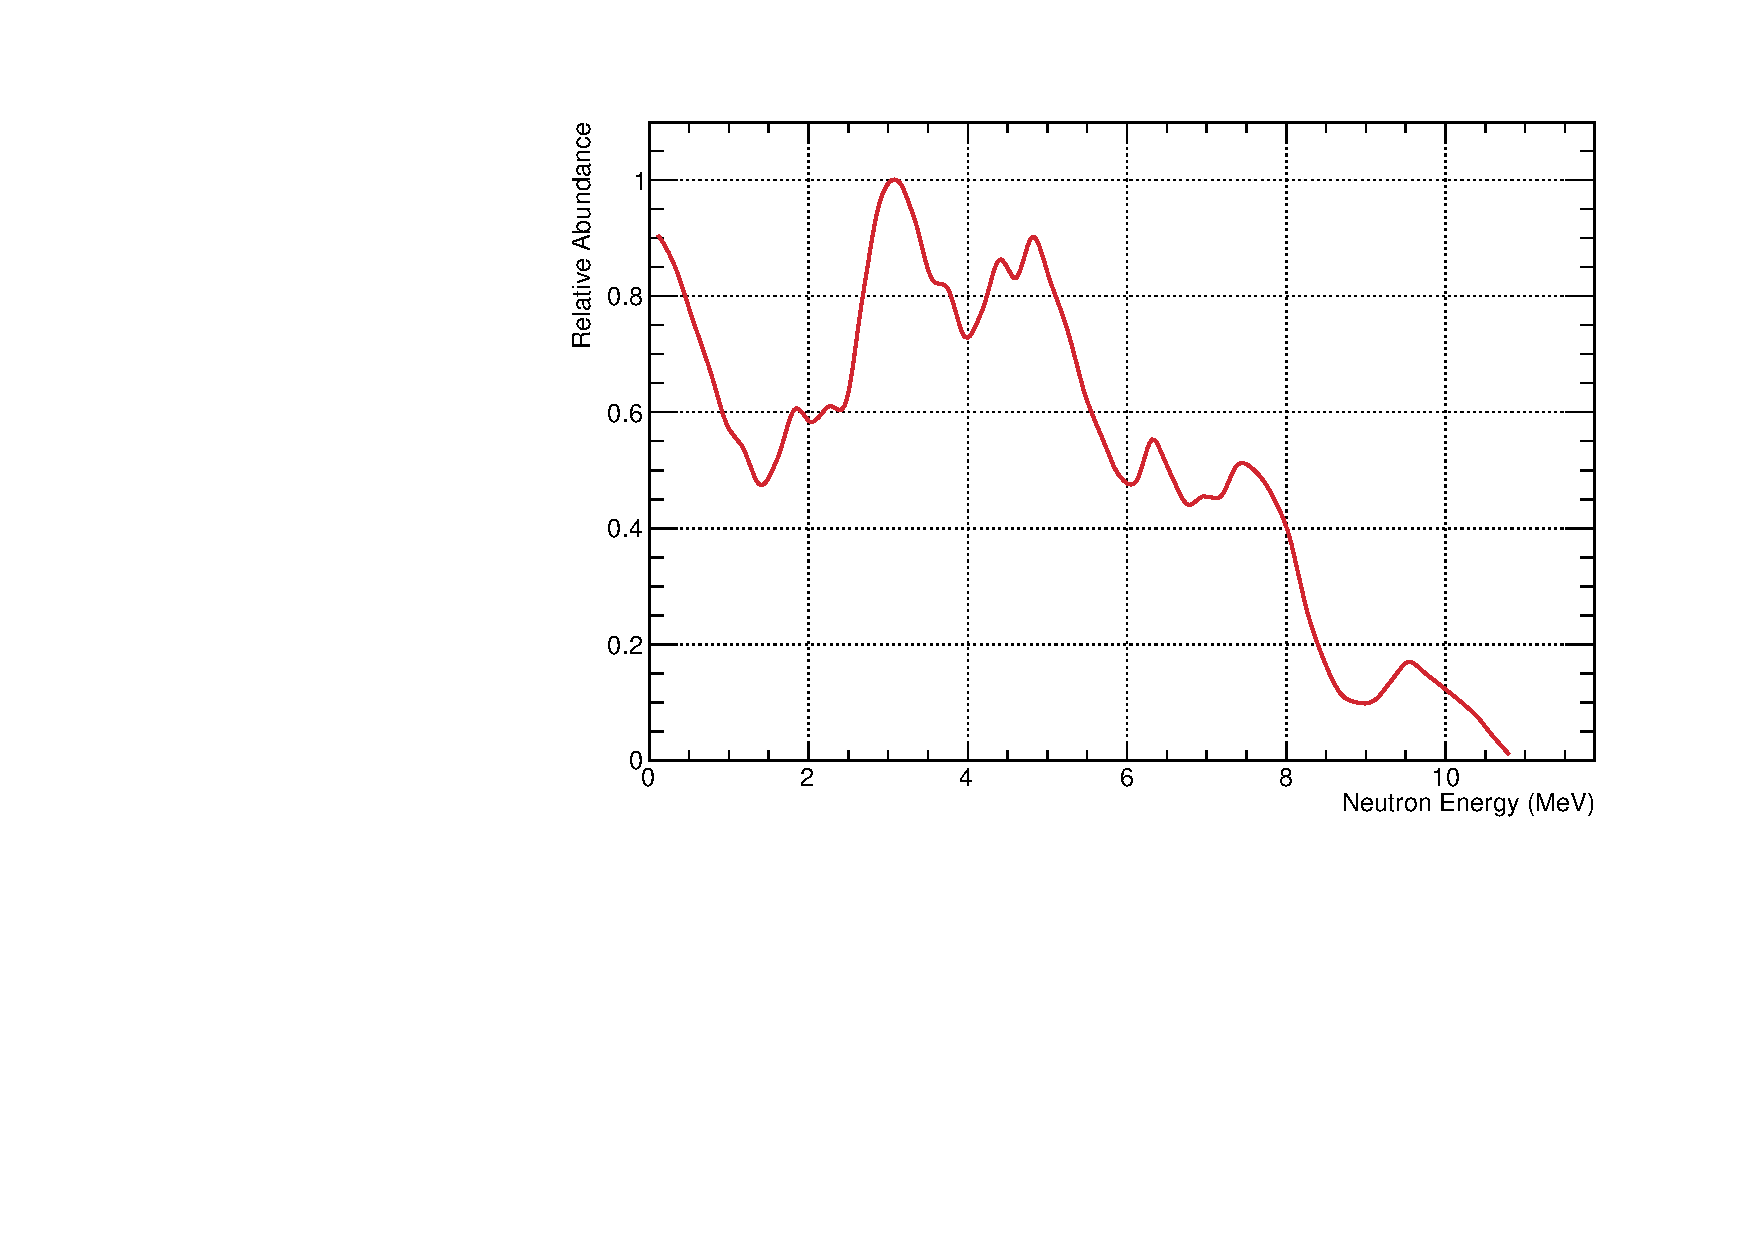
\includegraphics[trim={0 0 0 0.75cm},clip, width=\columnwidth]{images/AmBe_NeutronSpectrum.pdf}
	\caption[Energy spectrum of neutrons from AmBe source]{Energy spectrum of neutrons from AmBe source~\cite{AmBeSpec}.}
	\label{fig:AmBeSpec}
\end{figure}


\subsection{Helium-3 Tube}

\begin{figure}
	\centerfloat
		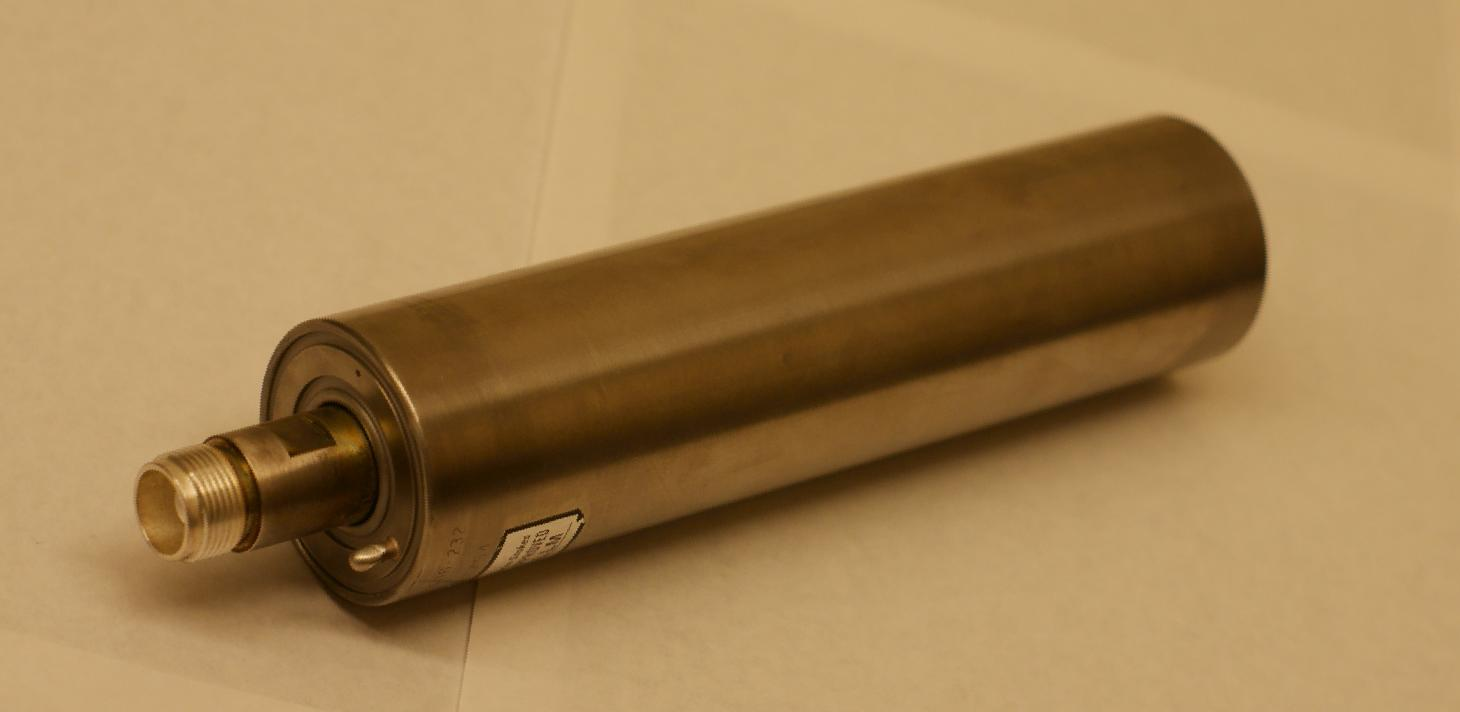
\includegraphics[width=\columnwidth]{images/he3tubePhoto}
	\caption[Helium-3 tube]{Helium-3 tube}
	\label{fig:he3photo}
\end{figure}


When a thermal neutron (with an energy of 0.025 eV) passes through the active area of the detector, it may be captured by a $^3$He atom~\cite{Oed200462}:

\begin{equation}
		{^{3}_{2}\mathrm{He}+^{1}_{0}\mathrm{n}\rightarrow~^{3}_{1}\mathrm{H}+^{1}_{1}H+764~\mathrm{keV}}
\end{equation}

The cross section for this reaction decreases as the energy of the neutron increases, as shown in Fig~\ref{fig:neutCross}. The $^3$H and proton ionize the gas in the tubes. This ionization produces a signal on a sense wire in the centre of the tube.

\begin{figure}
	\centerfloat
		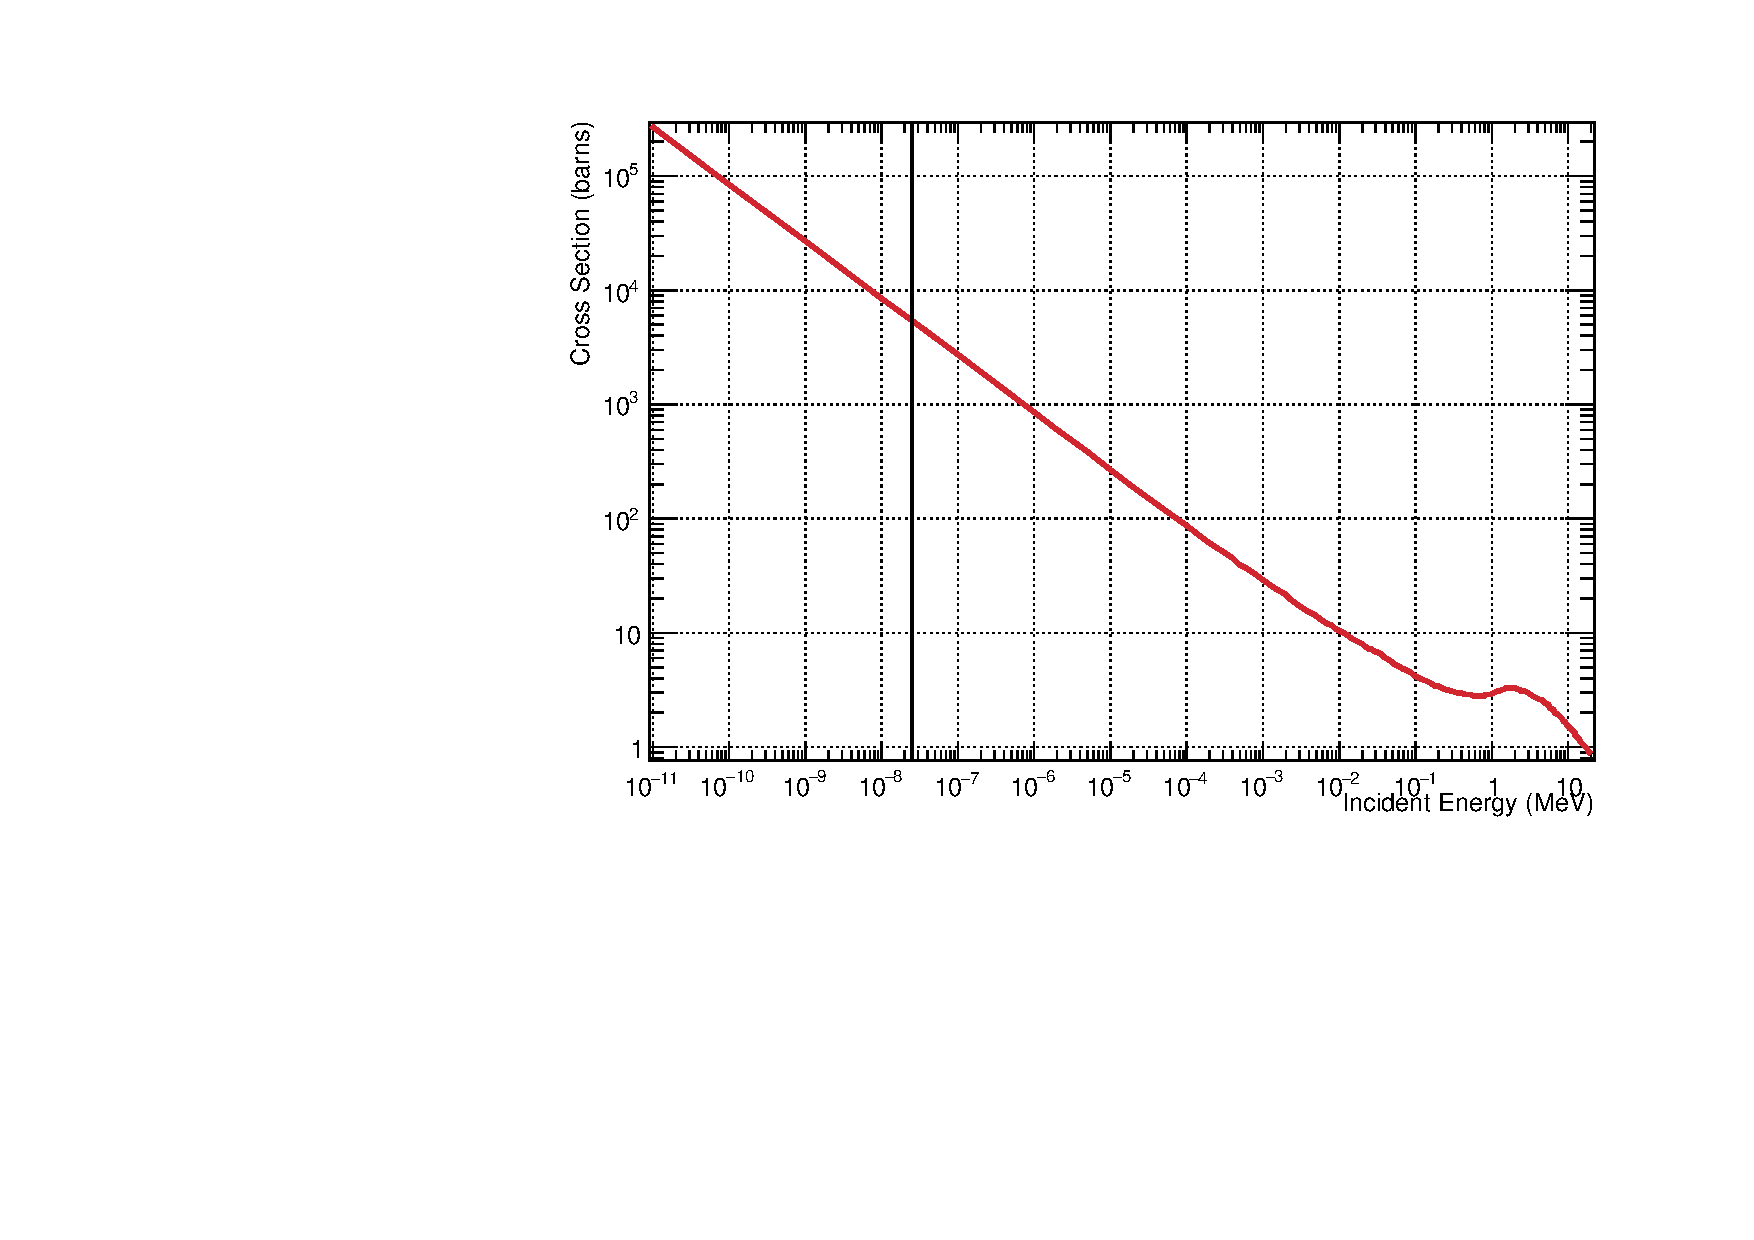
\includegraphics[width=\textwidth]{images/neutron_cross_section}
	\caption[Cross section of neutron capture by helium-3 as a function of neutron energy]{Cross section of neutron capture by helium-3 as a function of neutron energy. The vertical black line corresponds to upper range of the energy of thermal neutrons~\cite{BNL}.}
	\label{fig:neutCross}
\end{figure}



\section{Geometry}

	The centre of the geometry is defined to be the centre of the graphite cube. All other positions are taken relative to this point. The geometry of the pile room is read into the simulation from four files:

\begin{figure}
	\centerfloat
	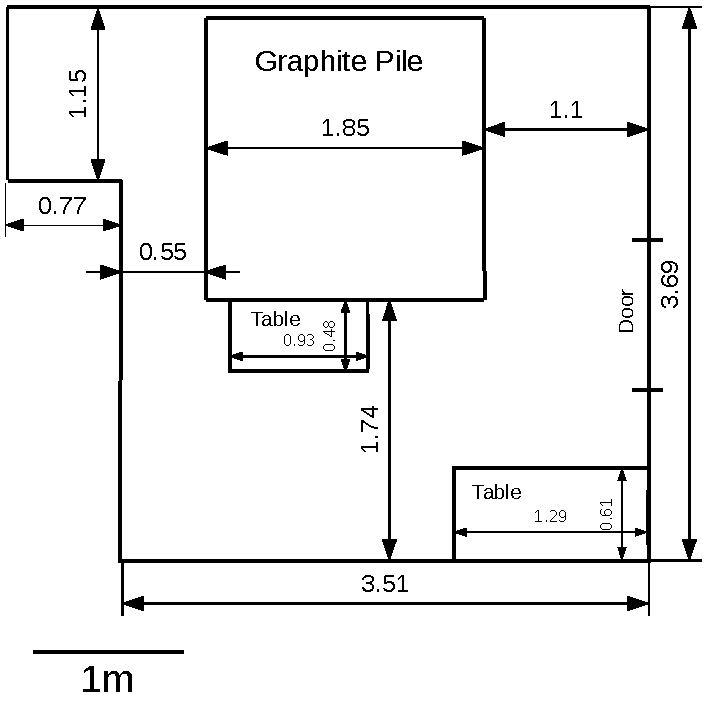
\includegraphics[width=\columnwidth]{images/Room}
	\caption{Scale drawing of the pile room}	
	\label{fig:room}
\end{figure}


\begin{figure}
	\centerfloat
	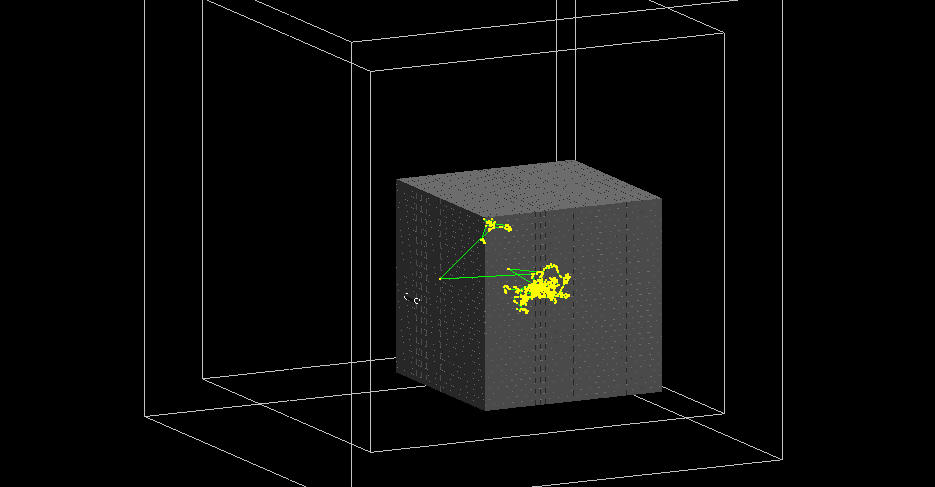
\includegraphics[width=\columnwidth]{images/10Events}
	\caption{Geometry as implemented in GEANT4. Yellow lines indicate the trajectory of a neutron event.}	
	\label{fig:tenEvents}
\end{figure}


	\paragraph{Room.xml} contains geometry of the room. The dimensions of the room, the material the walls are composed of, the thickness of the walls, and the position of the centre of the room relative to the graphite are all contained in this file. The default dimensions are taken from fig~\ref{fig:room}, the default 
material is G4\_CONCRETE, GEANT4's implementation of concrete, and the thickness is assumed to be 20cm. The door to the room and the small alcove on the left of fig~\ref{fig:room} have been omitted from the room description.

\begin{figure}
	\centerfloat
	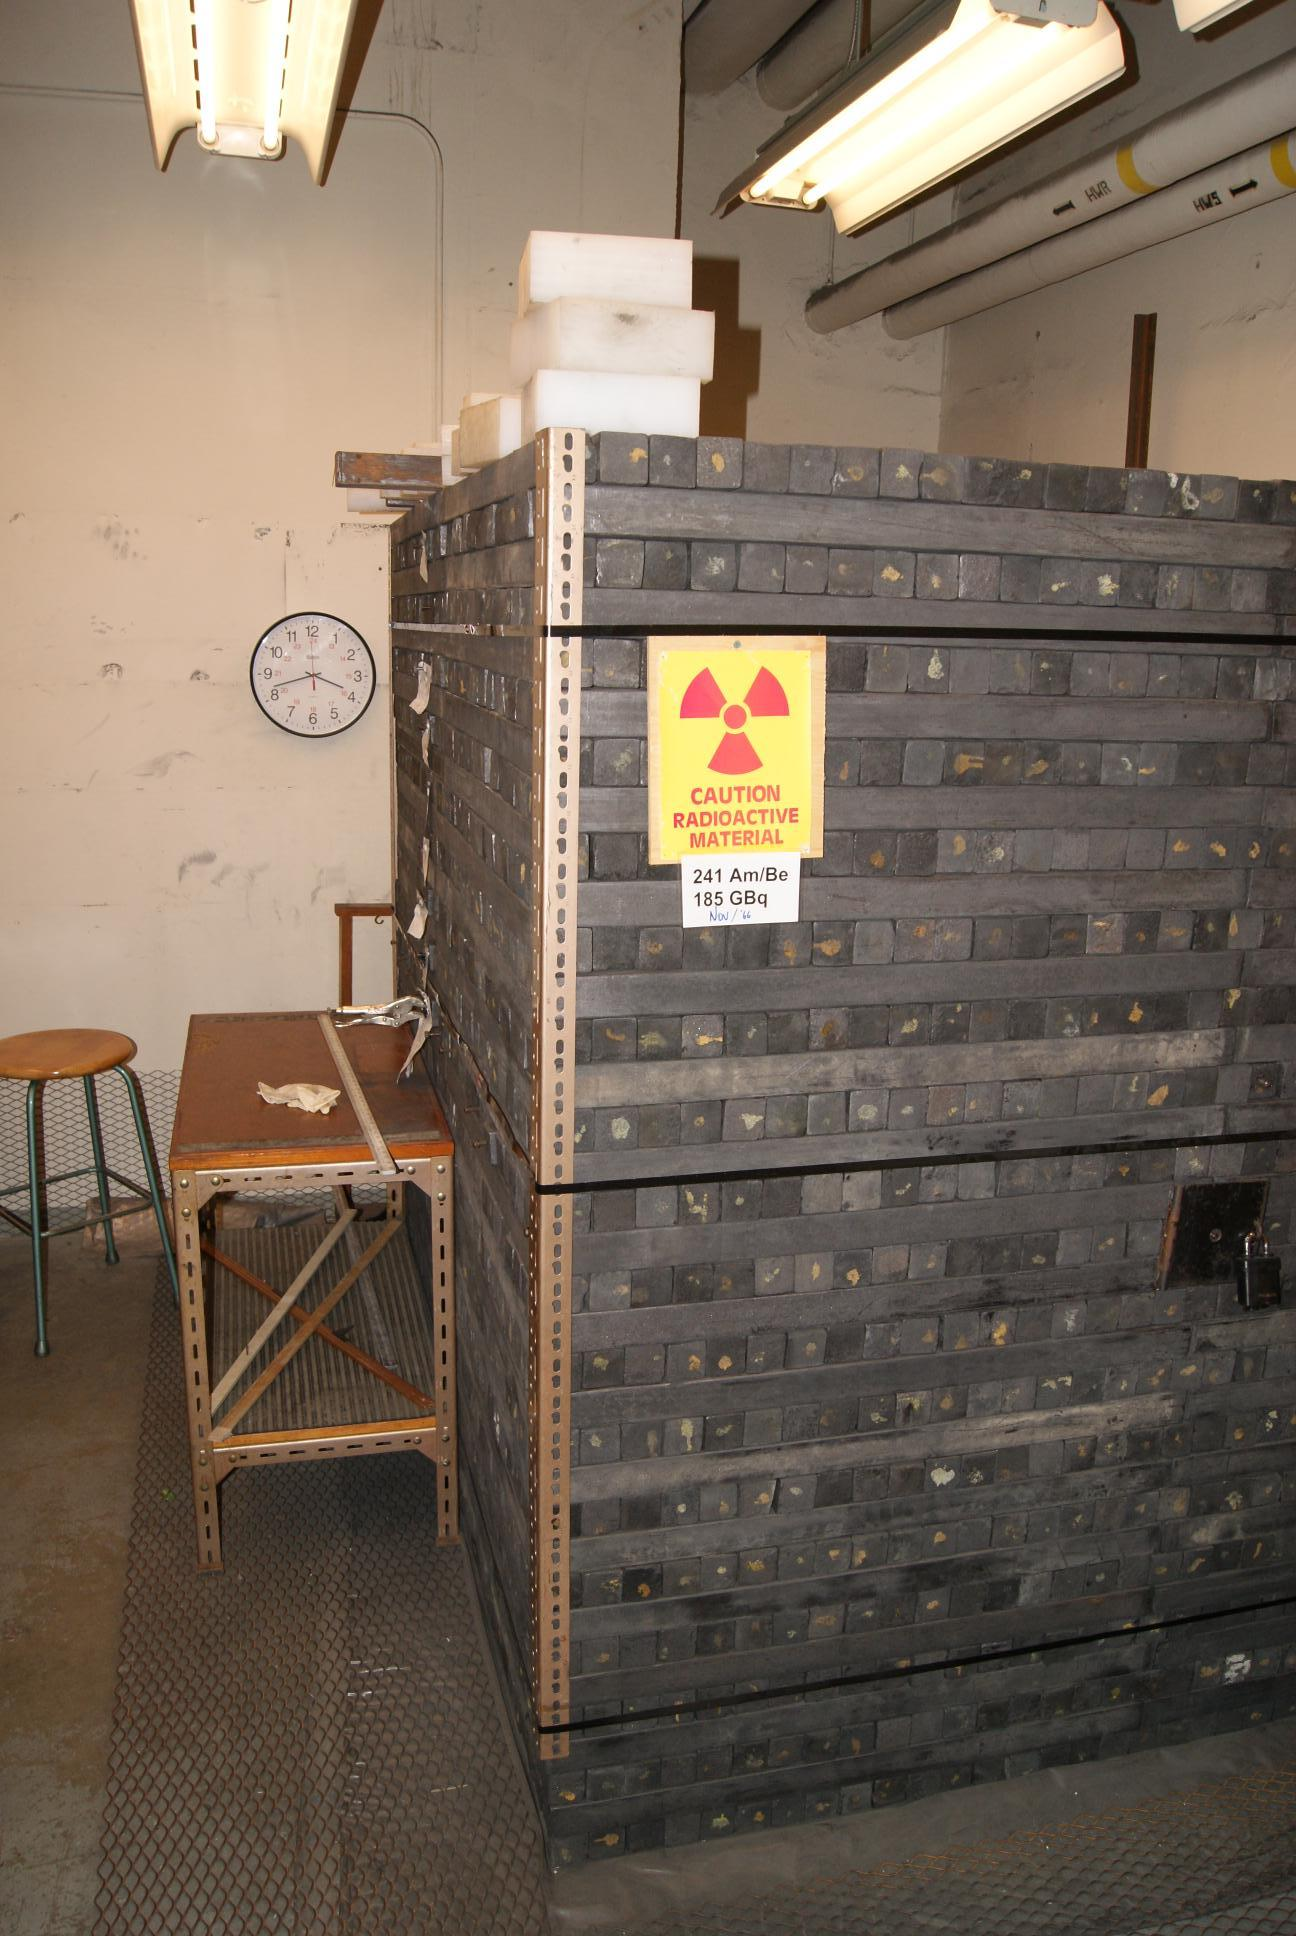
\includegraphics[width=0.5\columnwidth]{images/Rods}
	\caption{Photograph of the graphite pile showing rods}	
	\label{fig:graphiteRods}
\end{figure}

	\paragraph{Graphite.xml} contains the geometry of the graphite. The graphite pile is composed of layers of criss-crossed rods of graphite, as shown in fig~\ref{fig:graphiteRods}. 

	For simplicity, only the dimensions of one rod are defined in the xml file, as well as the number of layers in the pile. The default length of a rod is 92.5~cm with width of 5.285~cm. Each layer is two rods long and 35 wide, as shown in fig~\ref{fig:layers}, with each layer rotated 90$^{\circ}$ with respect to the previous. The pile is composed of 35 layers. The length and width if each rod is reduced by a Gaussian distributed random number in order to simulate the imperfect stacking and variation in rod dimensions of the actual pile. 

	The material of the pile is G4\_GRAPHITE with a small boron impurity. The density and the purity of the graphite (in \%) are specified in the xml file.


\begin{figure}
	\centerfloat
	\subfigure[layer 1]{
		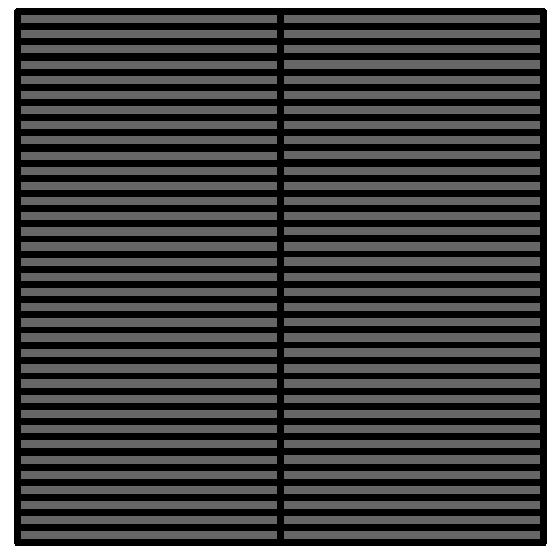
\includegraphics[width=0.5\columnwidth]{images/layer1}
	}
	\subfigure[layer 2]{
		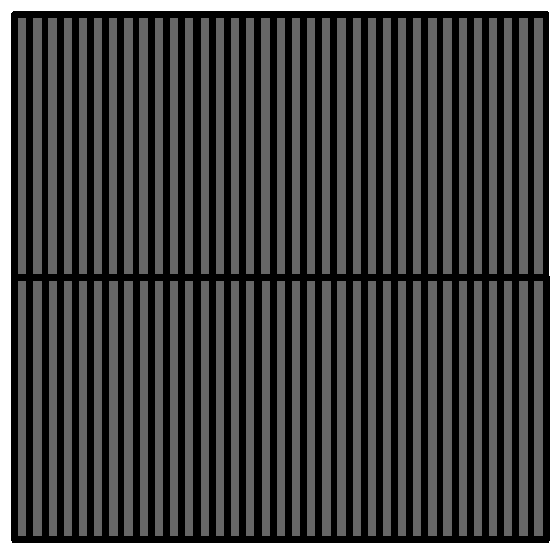
\includegraphics[width=0.5\columnwidth]{images/layer2}
	}
	\caption{Arrangement of rods in alternating layers}	
	\label{fig:layers}
\end{figure}


	\paragraph{HE3TUBE.xml} contains the geometry of the helium-3 tubes. The dimensions of the tubes are based on fig~\ref{fig:tubeSchematic}. The xml file can contain several tubes, each of which is implemented in the simulation.



	\paragraph{misc.xml} contains the geometry of any other object, such as a polyethylene shield. Both boxes and cylinders can be implemented. The position of the object can be with respect to the origin (the centre of the graphite) or with respect to one of the helium-3 tubes. The xml file can contan several objects, all of which will be implemented in the simulation.


\begin{figure}
	\centerfloat
	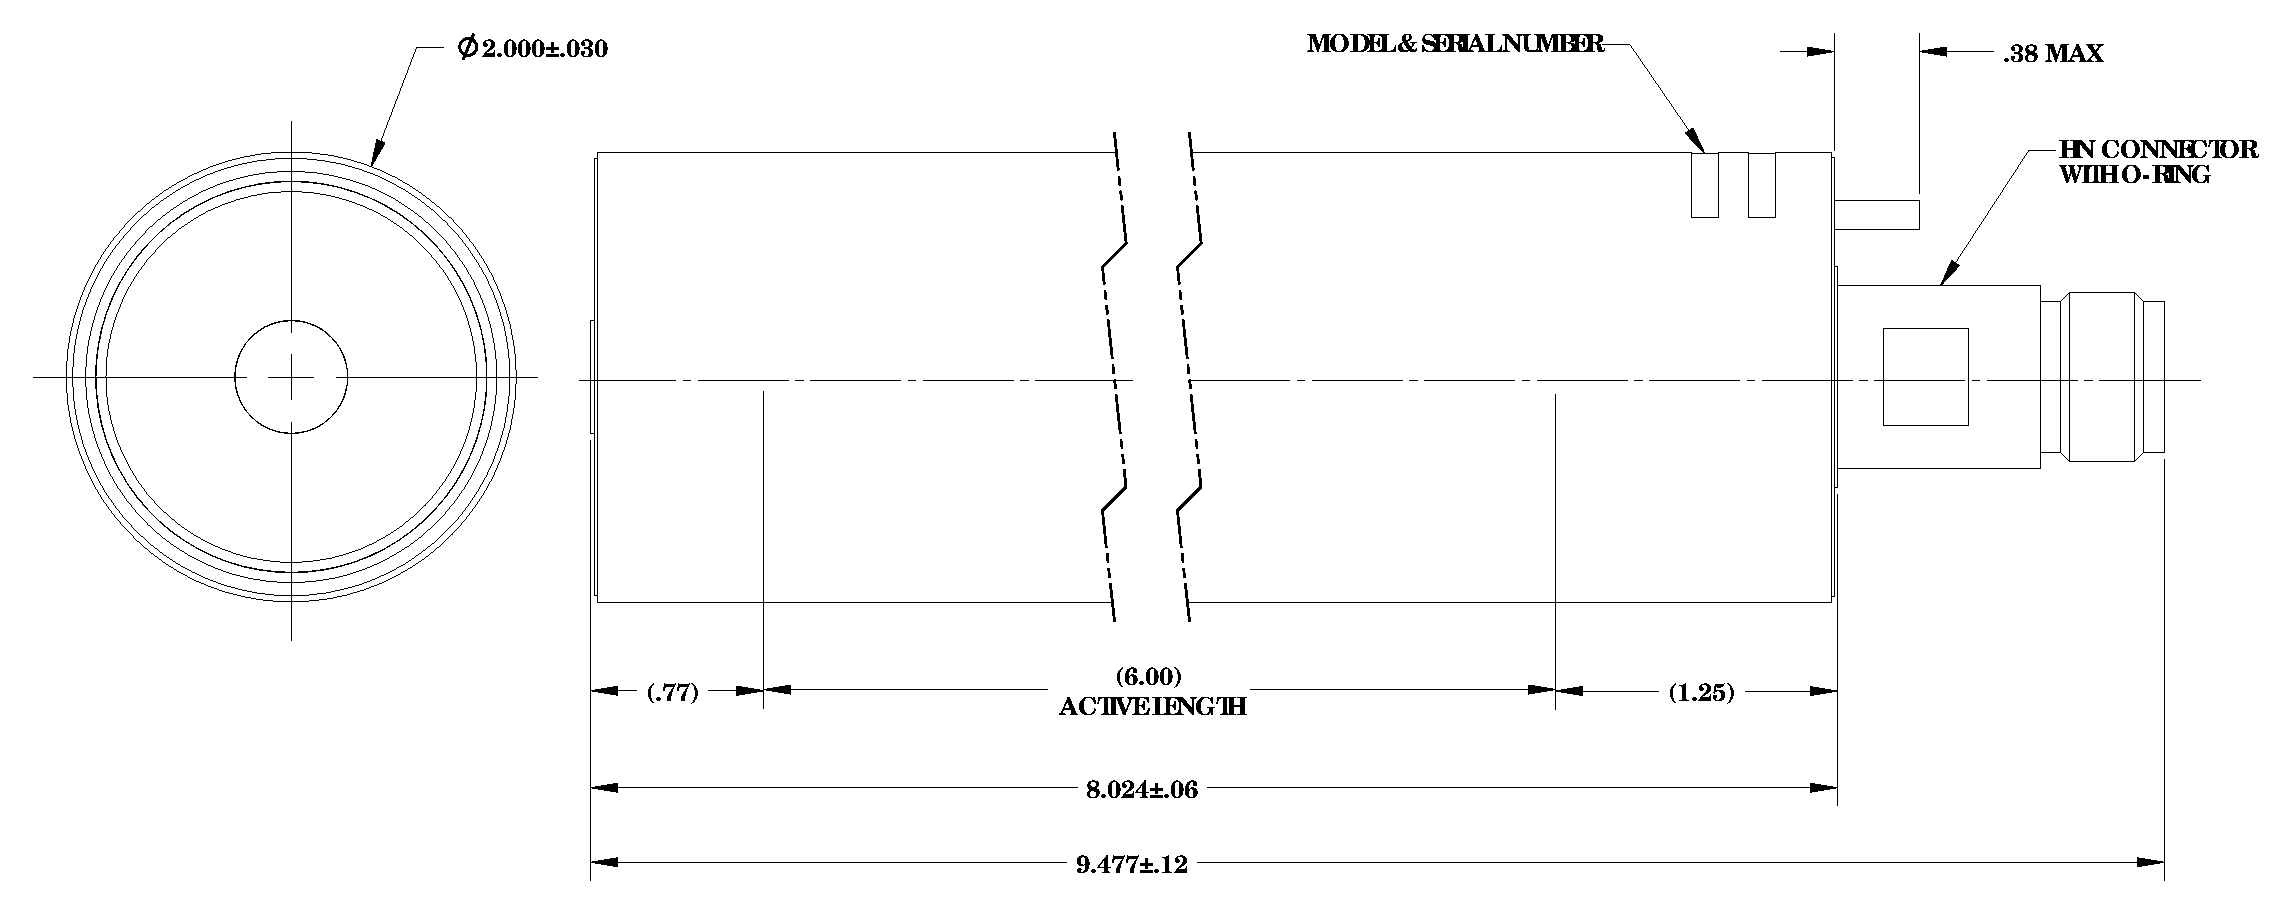
\includegraphics[width=\columnwidth]{images/GESchematic.pdf}
	\caption{Schematic of helium-3 tube}	
	\label{fig:tubeSchematic}
\end{figure}


\section{Output Ntuples}

	A root file containing two ntuples is produced by the simulation:

	\paragraph{geometry} contains the geometry of the room, graphite cube, helium-3 tubes, and the miscellaneous objects. This ntuple has only one entry.

	\paragraph{PileRoomSim} contains the simulation results. By default, only events containing a neutron hit in a helium-3 tube are saved, but it is possible to save all events. The branches in this ntuple summarized in table~\ref{tab:branches}

	
\begin{table}
	\centering
	\begin{tabular}{ rl }
		Branch	&	Description	\\	\hline	\hline
Ekin\_n\_PostGraphite	&	Kinetic energy of a neutron after leaving the graphite	\\		
Etot\_n\_initial	&	Initial energy of neutron	\\		
TotalEnergyDeposited	&	Total energy deposited by a proton and tritium	\\		
leftWall	&	1 if the neutron left the wall of the room	\\		
he3TubeXPos	&	X position of tube containing a neutron hit	\\		
he3TubeYPos	&	Y position of tube containing a neutron hit	\\		
he3TubeZPos	&	Z position of tube containing a neutron hit	\\		
EDEPinHe3	&	a vector of the energy deposits in the helium-3 tubes	\\		
PIDinHe3	&	a vector of the PID of particles causing energy deposits in 	\\		
	&	the helium-3 tubes	\\		
neutronHits	&	The channel number of a tube where a hit occured	\\		
diffusionRadius	&	a vector containing 100 radius values between 30 and 70~cm	\\		
diffusionFlux	&	a vector containing the number of neutrons which 	\\		
	&	cross a sphere defined by each entry in diffusionRadius	\\	\hline	

	
	\end{tabular}
	\caption{Branches in the PileRoomSim ntuple}
	\label{tab:branches}
\end{table}	




\section{Determination of Boron Contamination}

	Why??
\subsection{Diffusion length approach}

\begin{figure}
	\centerfloat
	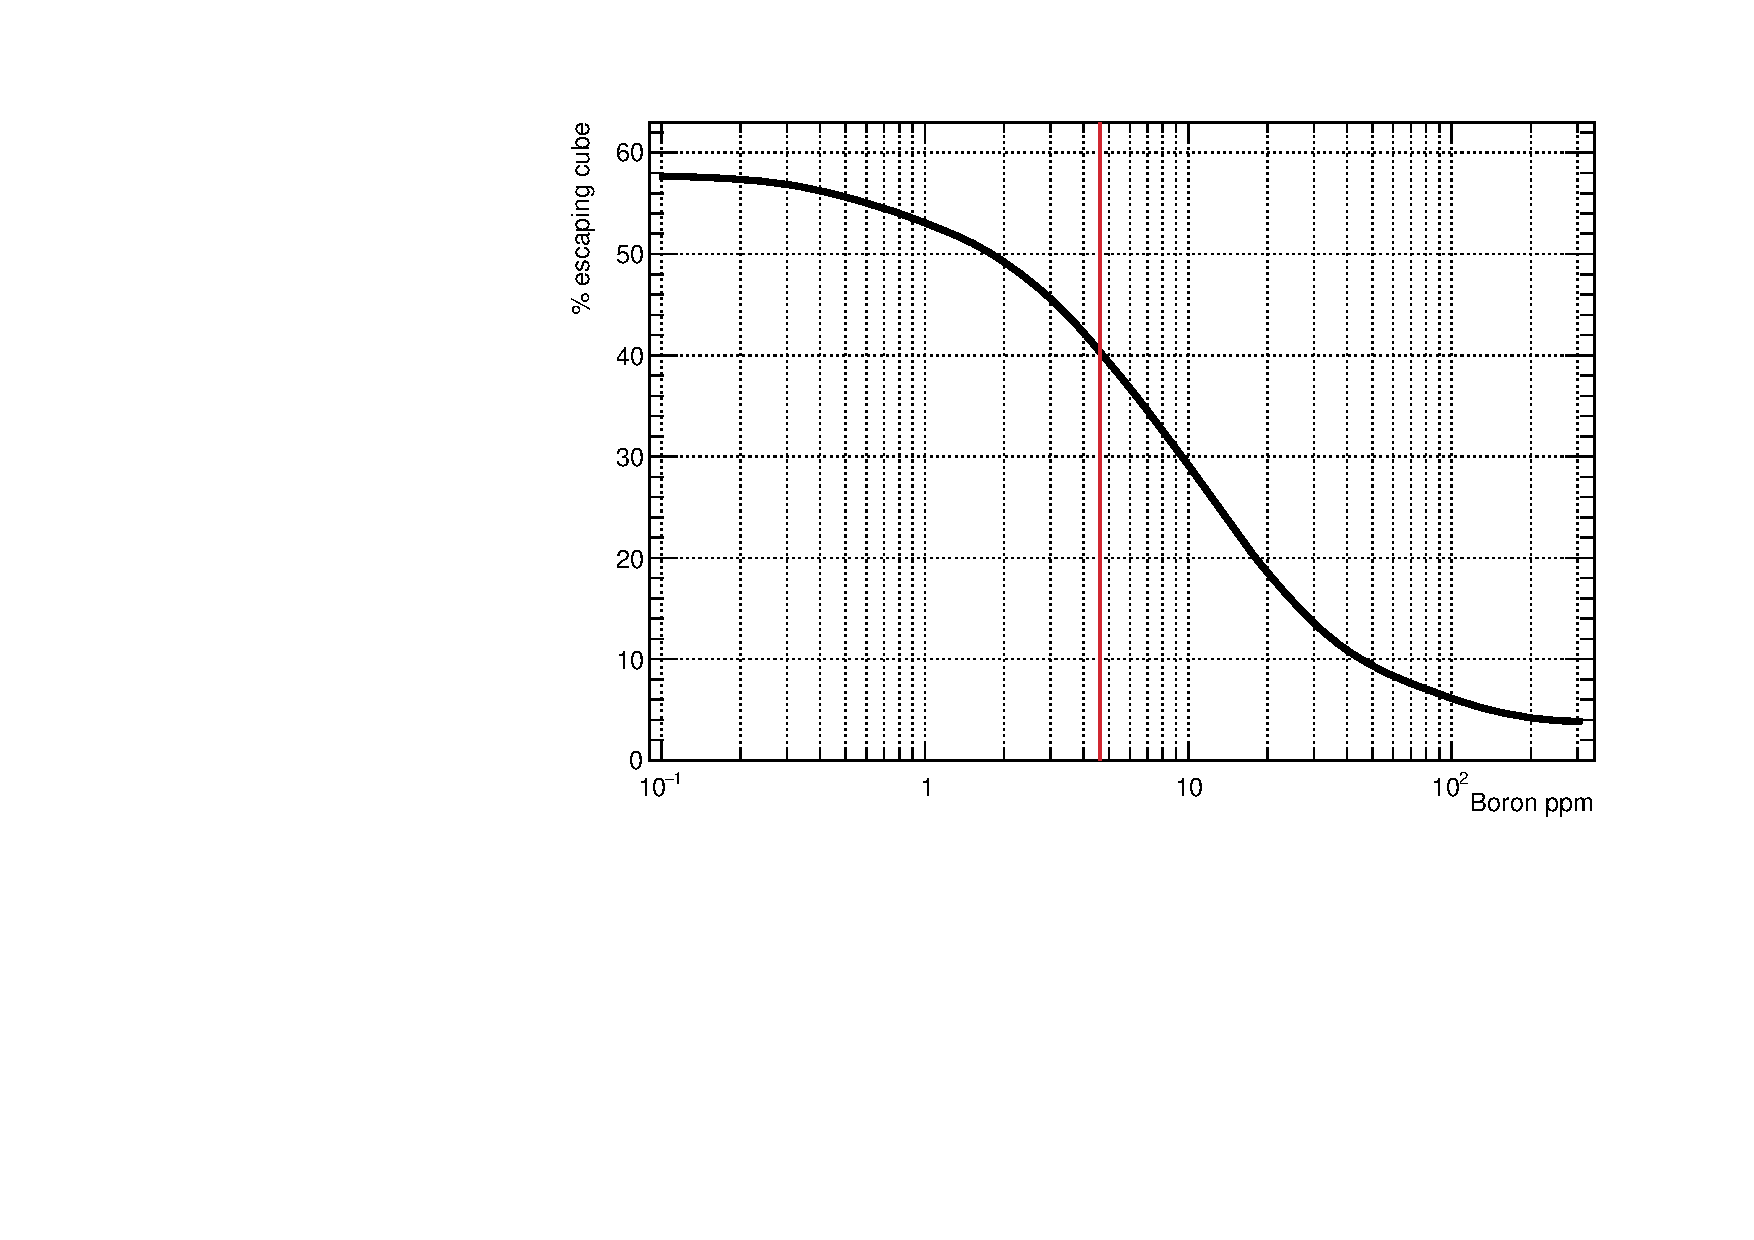
\includegraphics[width=\columnwidth]{images/BoronEscape}
	\caption{Fraction of neutrons which escape the graphite as a function of boron ppm}	
	\label{fig:boronExcape}
\end{figure}




	In the winter of 2017, and undergraduate student at UVic performed an experiment which measured the diffusion length of thermal neutrons in the graphite of the neutron source. The result of this experiment was a diffusion length of (0.429 $\pm$ 0.008)~m~\cite{undergradExpt}. The accepted value for the diffusion length on graphite is 0.503~m. I hypothesized that the difference between the measured value and the accepted value was due to a small boron impurity on the graphite. 




	I performed a measurement of the diffusion length in the simulated graphite pile. The diffusion length is related to the neutron flux by this relationship:
\begin{subequations}
\begin{align}
		{\phi = A\cdot exp(-\gamma r)}\\
		{\gamma^2 = 1/L^2}
\end{align}
\end{subequations}
Where $\phi$ is the neutron flux, $r$ is the distance from the source, and $L$ is the diffusion length.

	In the simulation the number of neutrons which enter or exit a shell of radius $r$ was counted, then divided by the surface area of the shell to get the neutron flux:
\begin{equation}
	{\phi = \frac{N_{\mathrm{neutrons}}} {4\pi r^2}   }
\end{equation}
This was plotted against the distance from the source (see fig~\ref{fig:neutronFlux}) was then fit to 
\begin{equation}
	{\phi = p_{0}\cdot exp(p_{1} r) + p_{2}}
\end{equation}
so that $L=1/p_{1}$. The range of $r$ was chosen so that a diffusion length of 0.503~m would be produced by pure graphite.



\begin{figure}
	\centerfloat
	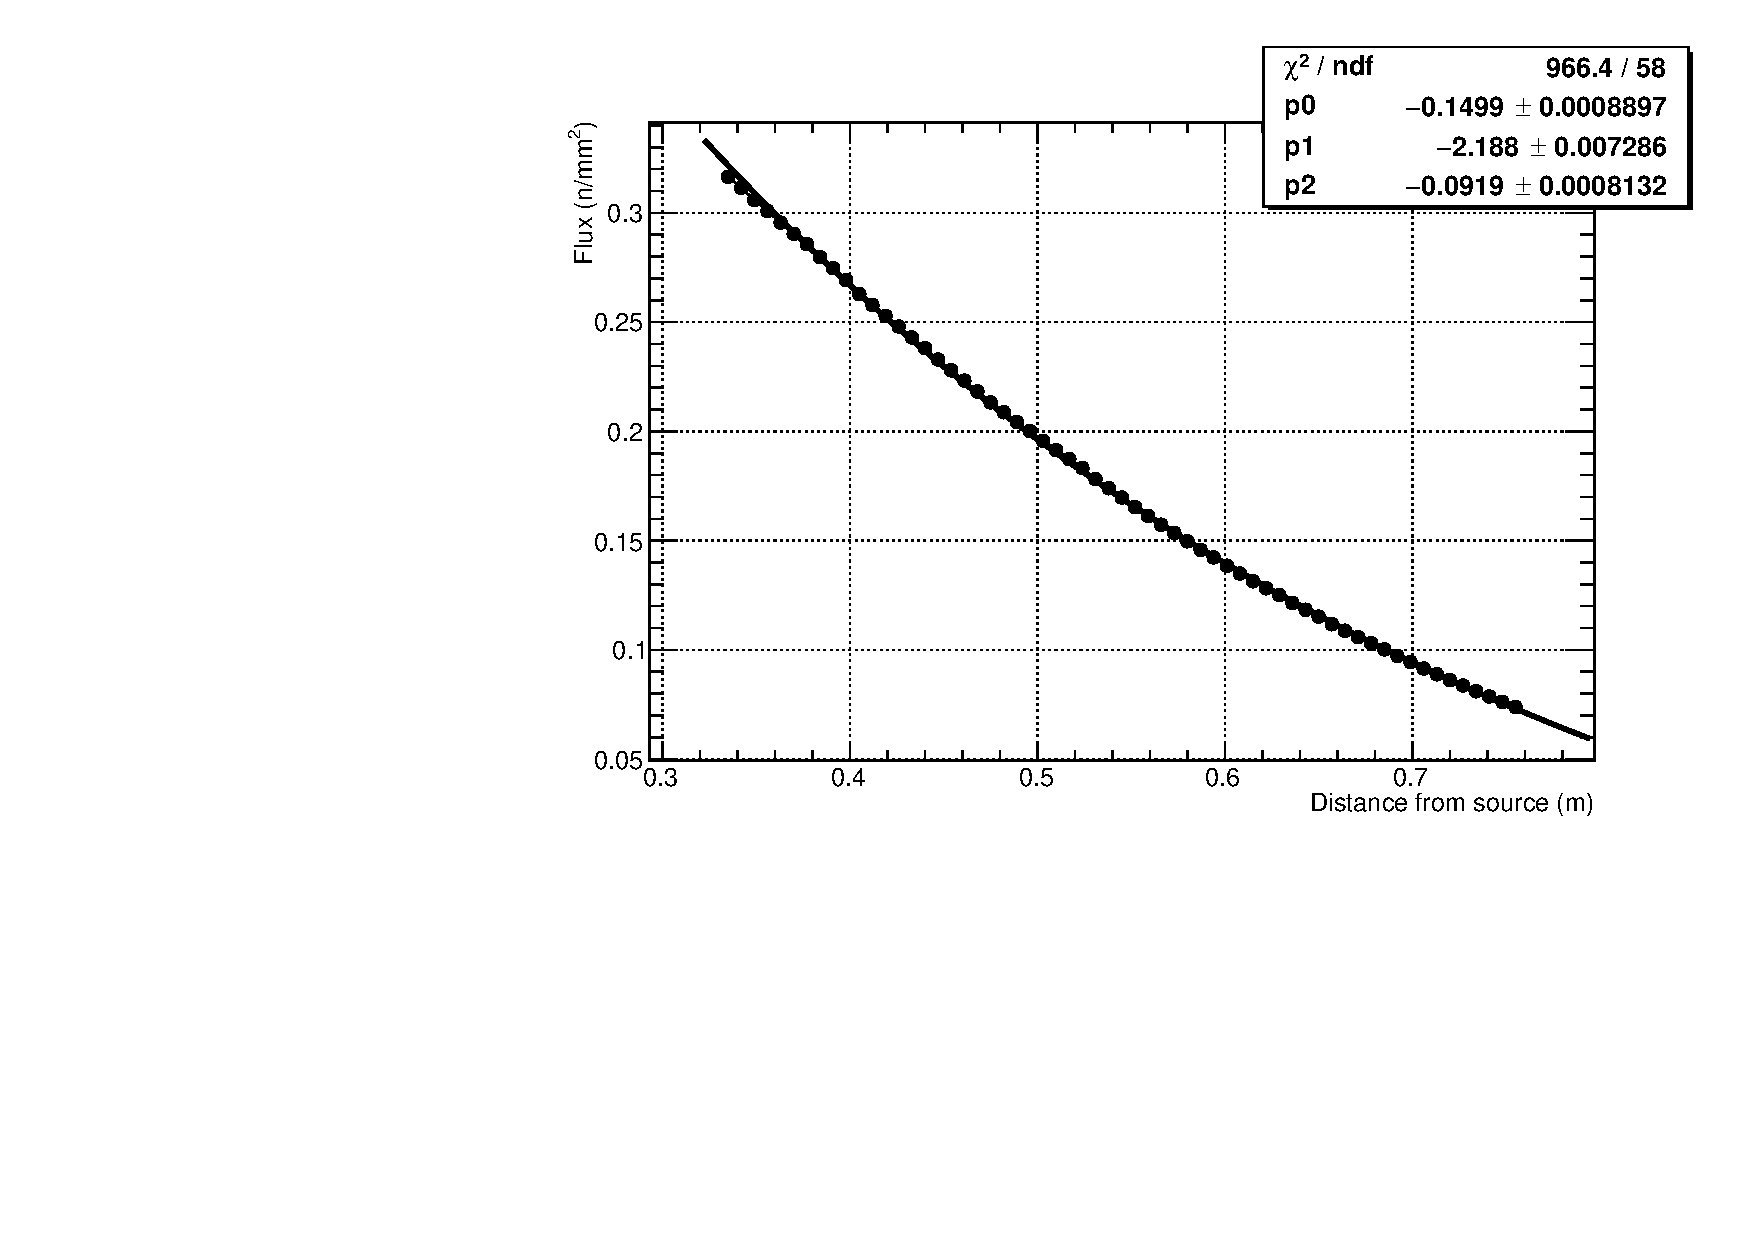
\includegraphics[width=\columnwidth]{images/fluxVsR}
	\caption{Neutron flux as a function of distance from the source for pure graphite}	
	\label{fig:neutronFlux}
\end{figure}


This process was repeated with boron impurites added (see fig~\ref{fig:neutronDiffLength}). The boron contamination which produced a diffusion length of 0.429~m was 4.63$\times10^{-4}$\% or 4.63 ppm boron.


\begin{figure}
	\centerfloat
	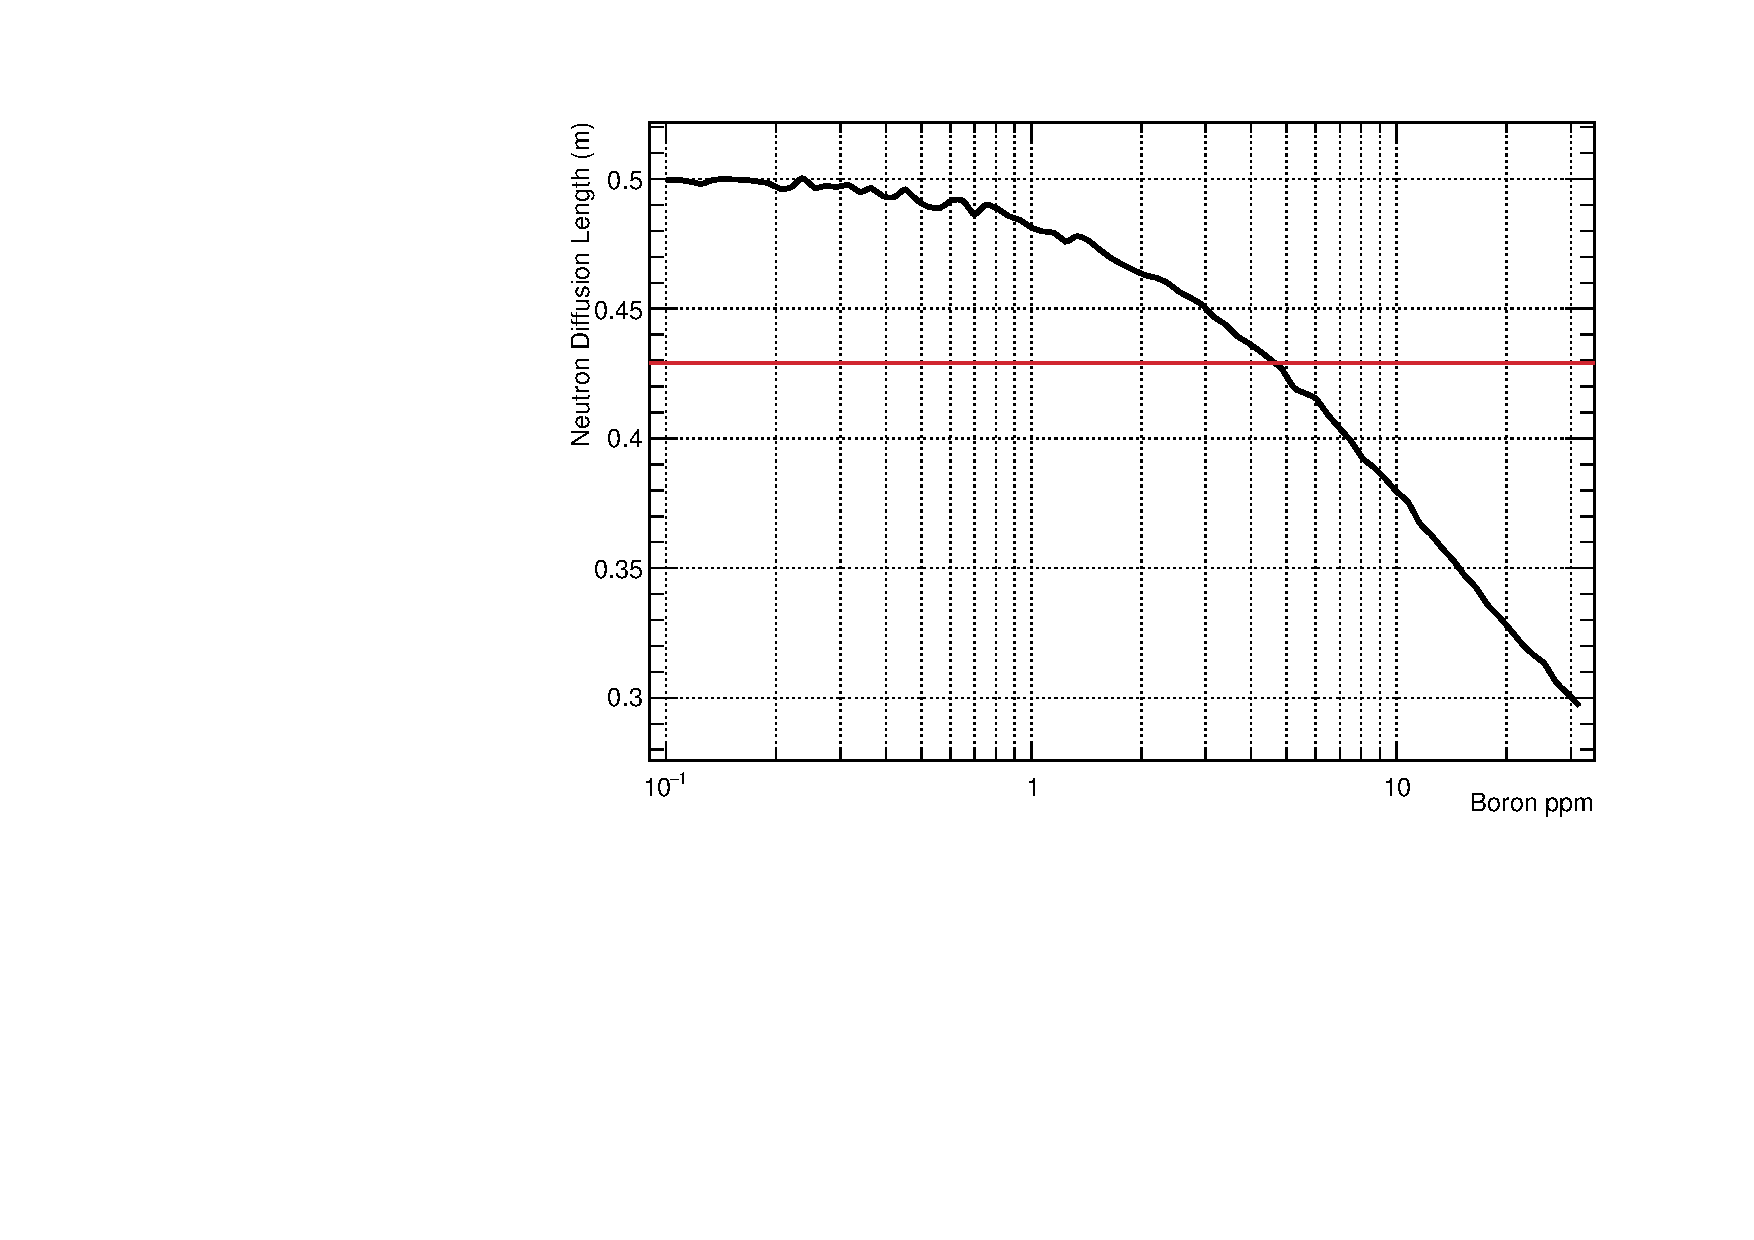
\includegraphics[width=\columnwidth]{images/DiffusionTuning_100}
	\caption{Neutron diffusion length as a function of boron contamination. The red line indicates the value of the diffusion length from the undergraduate experiment.}	
	\label{fig:neutronDiffLength}
\end{figure}


\subsection{Face measurement approach}


\begin{figure}
	\centerfloat
	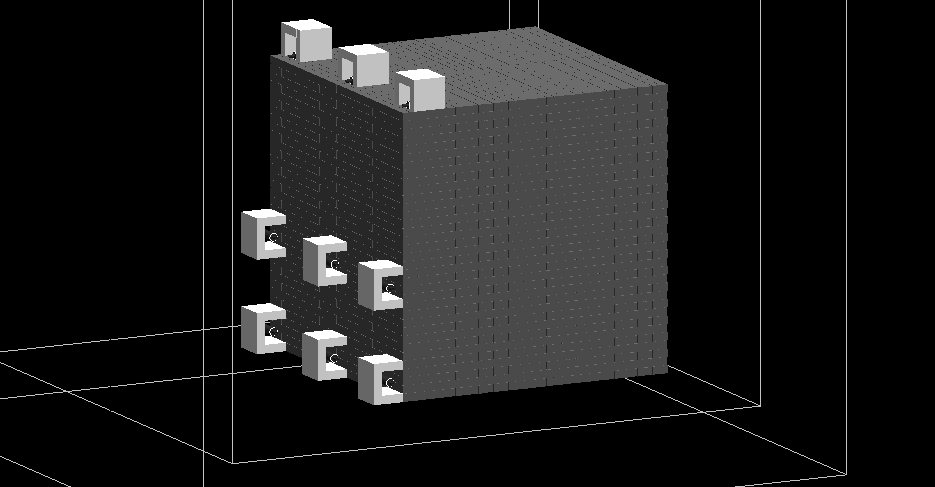
\includegraphics[width=\columnwidth]{images/FaceApproach}
	\caption{Locations of measurement on the face of the graphite. The white rectangles are polyethylene blocks to reduce the rate of neutrons from the walls.}	
	\label{fig:FaceImage}
\end{figure}

An alternative approach to determining the concentration of boron impurities was to measure the rate at different positions on the face of the graphite cube and compare with the simulated rate at the same positions. The positions measured and simulated can be seen in fig~\ref{fig:FaceImage}. The helium-3 tubes were surrounded with blocks of polyethylene to reduce the rate of neutrons bouncing back from the walls of the room.


The ratio of the rate at each position to the rate at the centre position was compared to the same ratio in simulation for a range of boron contamination. To determine the best fit between data and simulation, a $\chi^2$ analysis was used.






\clearpage
	\bibliographystyle{plain}
	\bibliography{References}




\end{document}
